%!TeX encoding=UTF-8
%!TeX root=main.tex
%!TeX program=xelatex

\documentclass[aspectratio=169]{beamer}

\usetheme[sectionpage=progressbar,subsectionpage=progressbar,numbering=fraction,
          progressbar=foot]{metropolis}

\graphicspath{{../img/}}
\usepackage{svg}

\usepackage{appendixnumberbeamer}

\usepackage{hyperref}

\usepackage{datetime}
\newdate{talkdate}{08}{03}{2018}

\usepackage[cache=false]{minted}
\usepackage{inconsolata}
\setmonofont{Inconsolata}

\usepackage{textcomp}

\usepackage{xpatch}
\usepackage[citestyle=authortitle,backend=bibtex]{biblatex}
\addbibresource{../bibl.bib}
\xapptobibmacro{cite}{\setunit{\nametitledelim}\printfield{year}}{}{}
\renewcommand{\footnotesize}{\scriptsize}

\title{Adaptating Amplified Unit Tests for Human Comprehension}

\date{\displaydate{talkdate}}
\author{%
  Simon Bihel\hfill\href{mailto:simon.bihel@ens-rennes.fr}{\nolinkurl{simon.bihel@ens-rennes.fr}}\\
}
\institute{%
  University of Rennes I \\
  \'Ecole Normale Sup\'erieure de Rennes
}

\begin{document}

\maketitle

\begin{frame}{Mutation Testing}
  \begin{columns}
    \begin{column}{0.7\textwidth}
      \minipage[c][0.7\textheight][s]{\columnwidth}
      Evaluating the quality of a test suite by injecting bugs
      \vfill{}
      Example of \emph{mutators}:
      \begin{itemize}
        \item change a \texttt{>} condition with \texttt{<};
        \item delete the body of a method.
      \end{itemize}
      \vfill{}
      \visible<2->{\textbf{Goal}\quad{} Enhance test suite by detecting new mutants}
      \endminipage{}
    \end{column}
    \begin{column}{0.3\textwidth}
      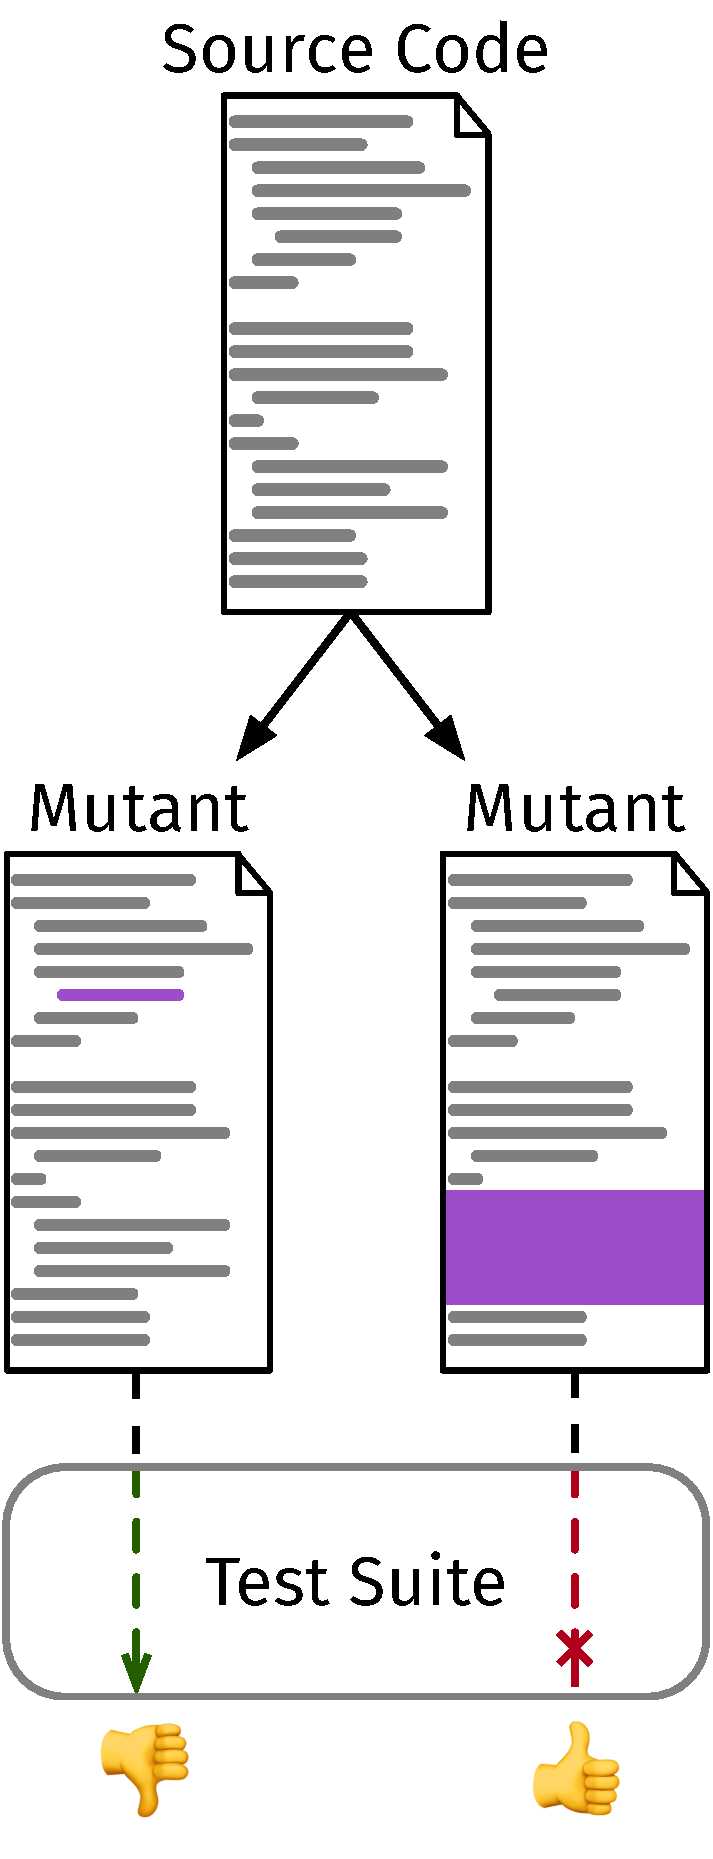
\includegraphics[height=\textheight]{mutation_testing}
    \end{column}
  \end{columns}
\end{frame}

\begin{frame}{DSpot\footnote{\url{https://github.com/STAMP-project/dspot}}}
  \begin{columns}
    \begin{column}{0.5\textwidth}
      Randomly modifies test cases:
      \begin{itemize}[<+(1)->]
        \item new inputs to trigger new behaviors;
        \item new assertions for unchecked properties;
        \item targets regression.
      \end{itemize}
    \end{column}
    \begin{column}{0.5\textwidth}
      \hspace*{-0.05\textwidth}
      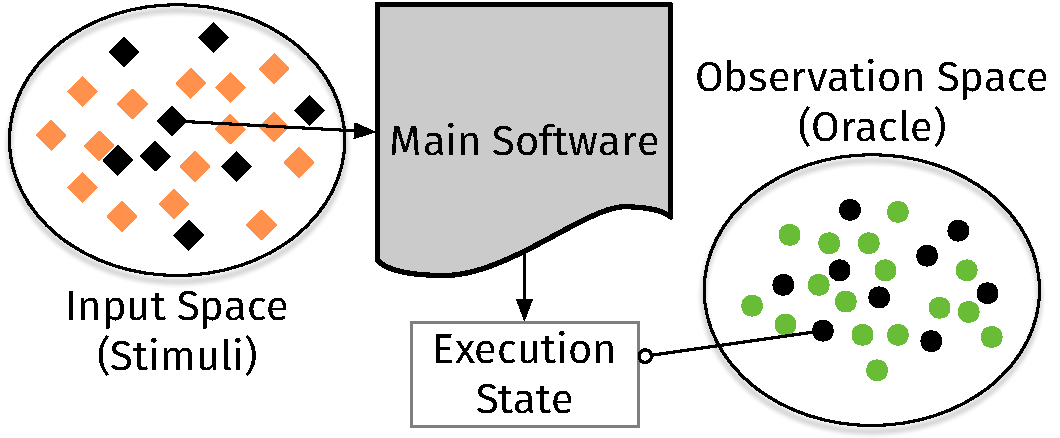
\includegraphics[width=1.1\textwidth]{spaces.pdf}
    \end{column}
  \end{columns}
  \vfill{}
  \visible<+->{Benjamin Danglot, INRIA Lille, France}
\end{frame}

\begin{frame}[fragile]{Example\footnote{\href{https://github.com/google/guava/blob/ea66419b6aa52678816df77caa304e617255cca5/guava-tests/test/com/google/common/graph/ImmutableGraphTest.java\#L29-L40}{https://github.com/google/guava/blob/master/guava-tests/test/com/google/common/graph/ImmutableGraphTest.java\#L29-L40}}}
  \begin{minted}[linenos]{java}
@Test
public void immutableGraph() {
  MutableGraph<String> mutableGraph = GraphBuilder.directed().build();
  mutableGraph.addNode("A");
  ImmutableGraph<String> immutableGraph = ImmutableGraph.copyOf(mutableGraph);

  assertThat(immutableGraph).isNotInstanceOf(MutableValueGraph.class);
  assertThat(immutableGraph).isEqualTo(mutableGraph);

  mutableGraph.addNode("B");
  assertThat(immutableGraph).isNotEqualTo(mutableGraph);
}
  \end{minted}
\end{frame}

\begin{frame}[fragile]{Example of amplification}
  \begin{minted}[linenos,highlightlines={5,9}]{java}
@Test
public void immutableGraph() {
  MutableGraph<String> mutableGraph = GraphBuilder.directed().build();
  mutableGraph.addNode("A");
  mutableGraph.addNode("C");
  ImmutableGraph<String> immutableGraph = ImmutableGraph.copyOf(mutableGraph);

  assertThat(immutableGraph).isNotInstanceOf(MutableValueGraph.class);
  assertTrue(immutableGraph.nodes().contains("A"));
  assertThat(immutableGraph).isEqualTo(mutableGraph);

  mutableGraph.addNode("B");
  assertThat(immutableGraph).isNotEqualTo(mutableGraph);
}
  \end{minted}
\end{frame}

\begin{frame}{Goal}
  \begin{itemize}
    \item Human-friendly, high-level, natural language description
  \end{itemize}
\end{frame}

\begin{frame}{Minimization}
  \begin{itemize}
    \item remove useless assertions
  \end{itemize}
\end{frame}

\begin{frame}{Slicing of Unit Tests}
  Simple static slicing
  \begin{itemize}
    \item Control-flow slicing
    \item Data-flow slicing
  \end{itemize}

  \begin{block}{Java tool}
    T.J. Watson Libraries for Analysis (WALA)\footnote{\url{https://github.com/wala/WALA}}
  \end{block}
\end{frame}

\begin{frame}{Natural Description}
  \begin{itemize}
    \item Mutator categorization
  \end{itemize}
\end{frame}

\end{document}
